%%%%%%%%%%%%%%%%%%%%%

%%%%%%%%%%%%%%%%%%%%%
\section{Cinemática}
La cinemática es la rama de la física que estudia el movimiento de los cuerpos sin considerar las causas que lo producen.

\begin{figure}[H]
    \centering
    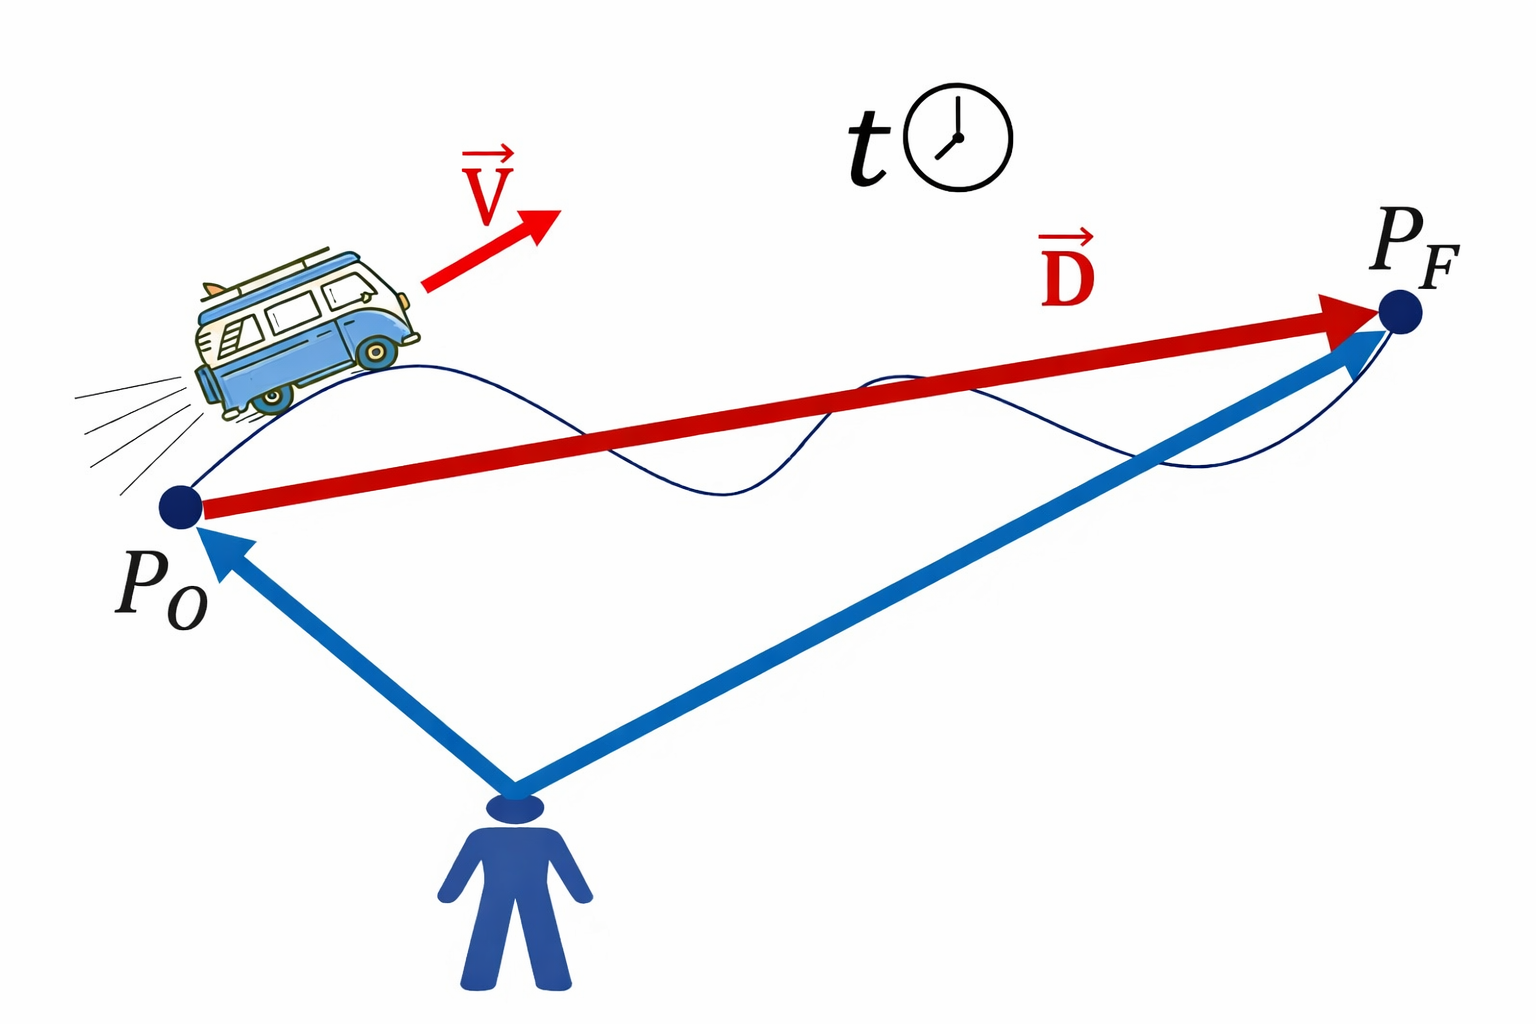
\includegraphics[width=0.5\textwidth]{images/cinematicImages/cinematic.png}
    \caption{Representación gráfica de la cinematica}
    \label{fig:cinematica}
\end{figure}

\vspace{-20pt}

\subsection{Sistema de referencia}
Es el marco o conjunto de coordenadas desde el cual un observador describe la posición y el movimiento de un objeto. Permite establecer medidas de distancia, dirección y tiempo.

\begin{figure}[H]
    \centering
    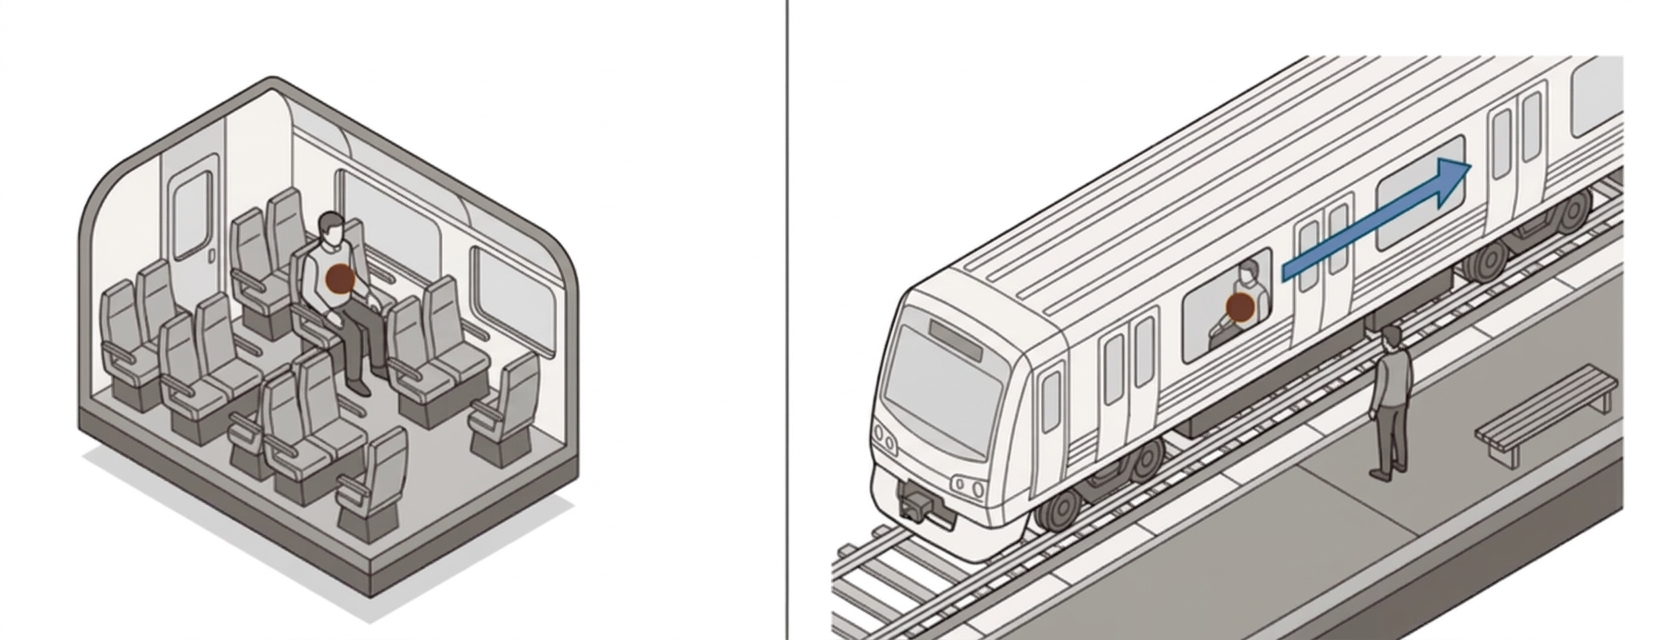
\includegraphics[width=0.6\textwidth]{images/cinematicImages/referenceSystem.png}
    \caption{Representación gráfica del sistema de referencia}
    \label{fig:sistemaDeReferencia}
\end{figure}

\vspace{-20pt}

\subsubsection{Observador interno}
Es aquel que se encuentra dentro del sistema en movimiento, es decir, forma parte del cuerpo que se desplaza. Desde su perspectiva, los objetos que se mueven junto a él parecen estar en reposo, mientras que los elementos externos aparentan moverse en sentido contrario.

\subsubsection{Observador externo}
Es aquel que se encuentra fuera del sistema en movimiento, observando el desplazamiento desde un punto fijo. Desde su perspectiva, puede apreciar con claridad la trayectoria, la velocidad y los cambios de posición del cuerpo en movimiento.

\subsection{Posición}
La posición de un objeto indica su ubicación en el espacio respecto a un punto del sistema de referencia (origen). Se representa generalmente con la variable $x$ para el caso unidimensional.

\begin{itemize}
    \item \textbf{En una dimensión (1D):} la posición se describe mediante una sola coordenada, generalmente $x$, que indica la distancia (con signo) respecto al origen.
    
    \item \textbf{En dos dimensiones (2D):} la posición se describe mediante un vector $\vec{r}$ compuesto por dos coordenadas, $x$ e $y$, que determinan la ubicación del objeto en el plano.
\end{itemize}

\begin{figure}[H]
    \centering
    \begin{subfigure}{0.4\textwidth}
        \centering
        \includegraphics[width=\linewidth]{images/cinematicGraphics/1DPosition.jpg}
        \caption{Posición en "1D"}
    \end{subfigure}
    \hspace{0.02\textwidth}
    \begin{subfigure}{0.4\textwidth}
        \centering
        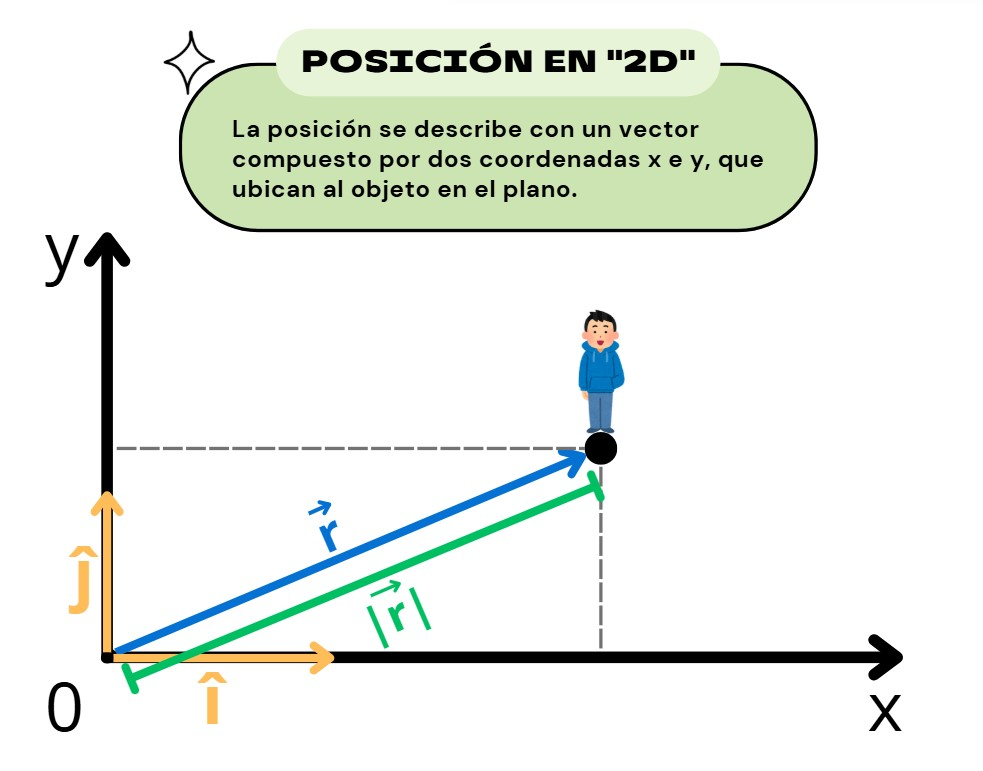
\includegraphics[width=\linewidth]{images/cinematicGraphics/2DPosition.jpg}
        \caption{Posición en "2D"}
    \end{subfigure}
    \caption{Representaciones gráficas de las posiciones}
    \label{fig:posiciones}
\end{figure}

\vspace{-40pt}

\[
\begin{array}{l@{\hspace{5cm}}l}

\colorbox{blue!20}{$\vec{r} = x_0(\pm \hat{\imath})$}
&
\colorbox{blue!20}{$\vec{r} = x\hat{\imath} + y\hat{\jmath}$}
\\&
\colorbox{blue!20}{$|\vec{r}| = \sqrt{x^2 + y^2}$}
\\

\end{array}
\]

\[
[\vec{r}\,] = [\mathrm{m}] \quad \text{S.I.} 
\]

\subsection{Desplazamiento}
El desplazamiento es la variación de posición de un objeto entre dos instantes de tiempo.

\begin{figure}[H]
    \centering
    \begin{subfigure}{0.4\textwidth}
        \centering
        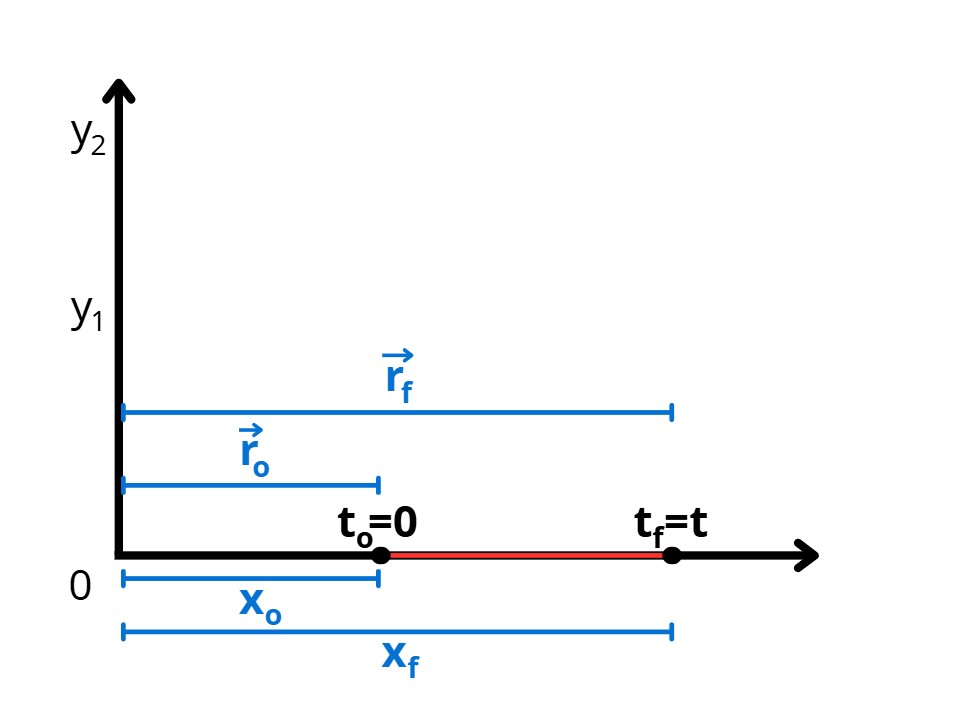
\includegraphics[width=\linewidth]{images/cinematicGraphics/1DDisplacement.jpg}
        \caption{Desplazamiento en "1D"}
    \end{subfigure}
    \hspace{0.02\textwidth}
    \begin{subfigure}{0.4\textwidth}
        \centering
        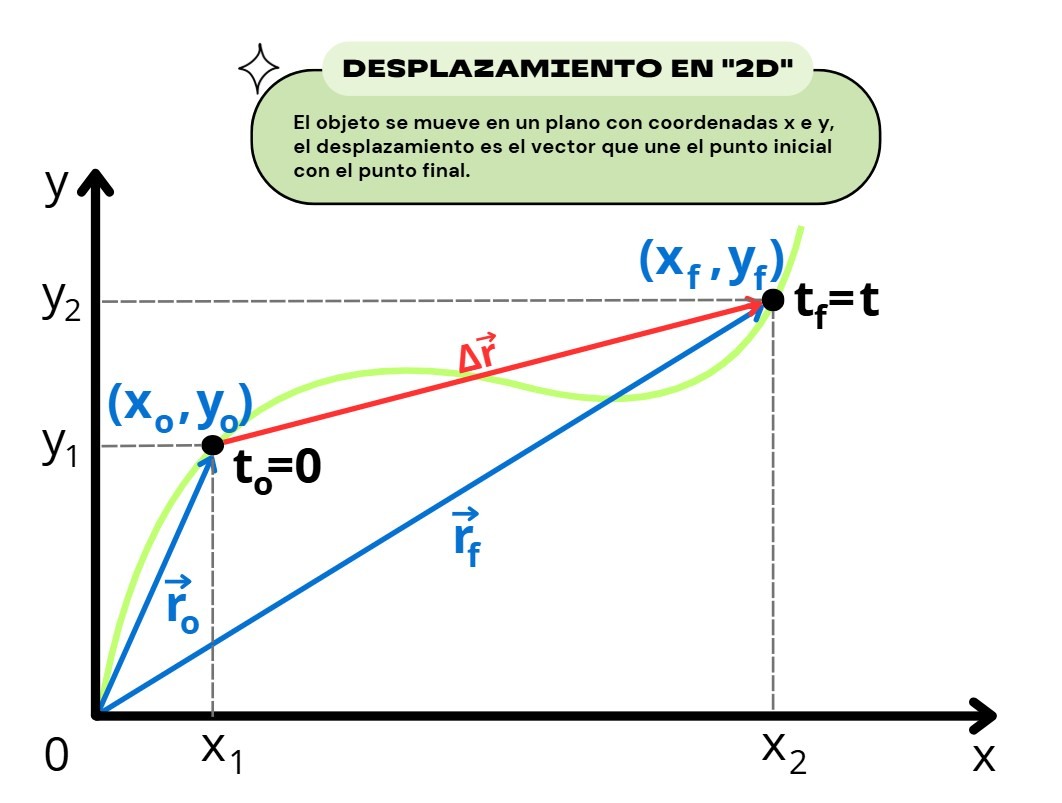
\includegraphics[width=\linewidth]{images/cinematicGraphics/2DDisplacement.jpg}
        \caption{Desplazamiento en "2D"}
    \end{subfigure}
    \caption{Representaciones gráficas de los desplazamientos}
    \label{fig:desplazamiento}
\end{figure}

\vspace{-50pt}

\[
\begin{array}{l@{\hspace{5cm}}l}

\colorbox{blue!20}{$\Delta \vec{x} = \vec{x}_f - \vec{x}_o$}
&
\colorbox{blue!20}{$\Delta \vec{r} = \vec{r}_f - \vec{r}_o$}
\\&
\vec{r}_o = x_o \hat{\imath} + y_o \hat{\jmath}
\\&
\vec{r}_f = x_f \hat{\imath} + y_f \hat{\jmath}
\\

\end{array}
\]

\vspace{-15pt}

\[
[\Delta \vec{r}\,] = [\mathrm{m}] \quad \text{S.I.} 
\]

Donde $x_f$ es la posición final y $x_0$ es la posición inicial. A diferencia de la distancia recorrida, el desplazamiento puede ser positivo, negativo o cero.

\subsection{Velocidad y rapidez}

\begin{figure}[H]
    \centering
    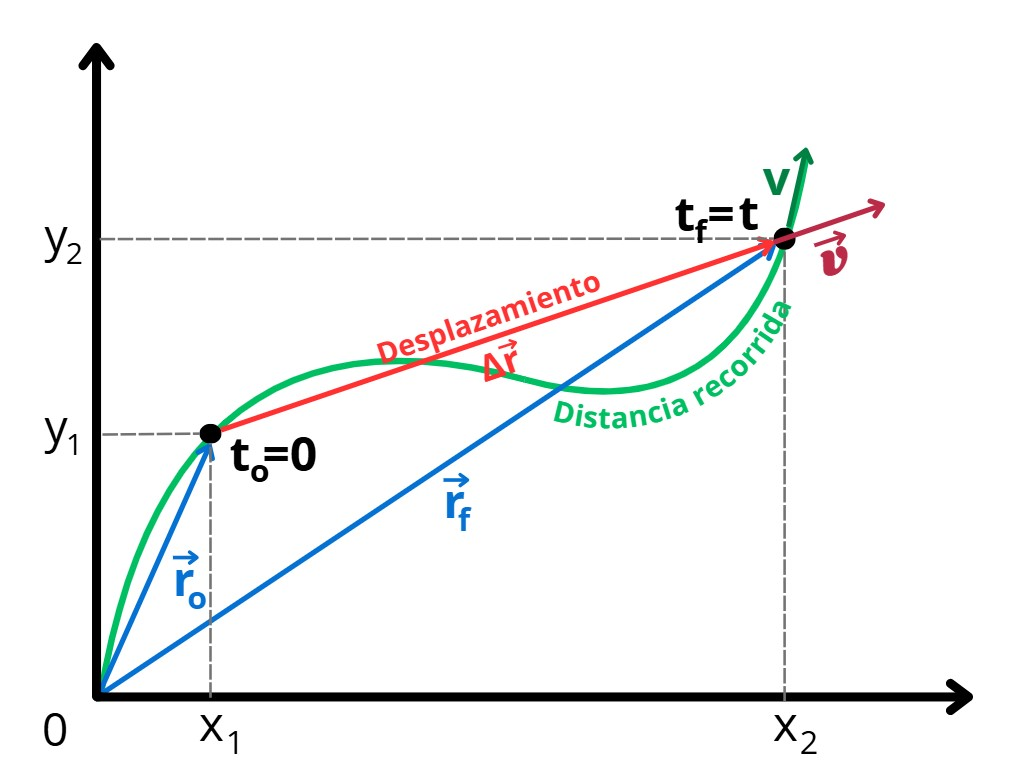
\includegraphics[width=0.6\textwidth]{images/cinematicGraphics/speedAndSpeed.jpg}
    \caption{Representación gráfica de la velocidad y rapidez}
    \label{fig:velocidad y rapidez}
\end{figure}

\vspace{-20pt}

\subsubsection{Velocidad}
La velocidad es una magnitud vectorial que expresa la variación de posición por unidad de tiempo. A diferencia de la rapidez, considera la dirección y el sentido del movimiento.

\[
\text{velocidad} = \frac{\text{desplazamiento}}{t} = \frac{\Delta{x}}{t}
\]

\vspace{-10pt}

\[
\colorbox{blue!20}{$\displaystyle {v} = \frac{\Delta x}{t}$}
\]

\subsubsection{Rapidez}

La rapidez es una magnitud escalar que indica qué tan rápido se mueve un objeto.

\[
\text{rapidez} = \frac{\text{distancia recorrida}}{t} = \frac{\text{d}}{t}
\]

\vspace{-10pt}

\[
\colorbox{blue!20}{$\displaystyle \text{v} = \frac{\text{d}}{t}$}
\]

\subsection{Velocidad media e instantánea}

\subsubsection{Velocidad media}
La velocidad media es el cociente entre el desplazamiento total y el intervalo de tiempo correspondiente:

\begin{figure}[H]
    \centering
    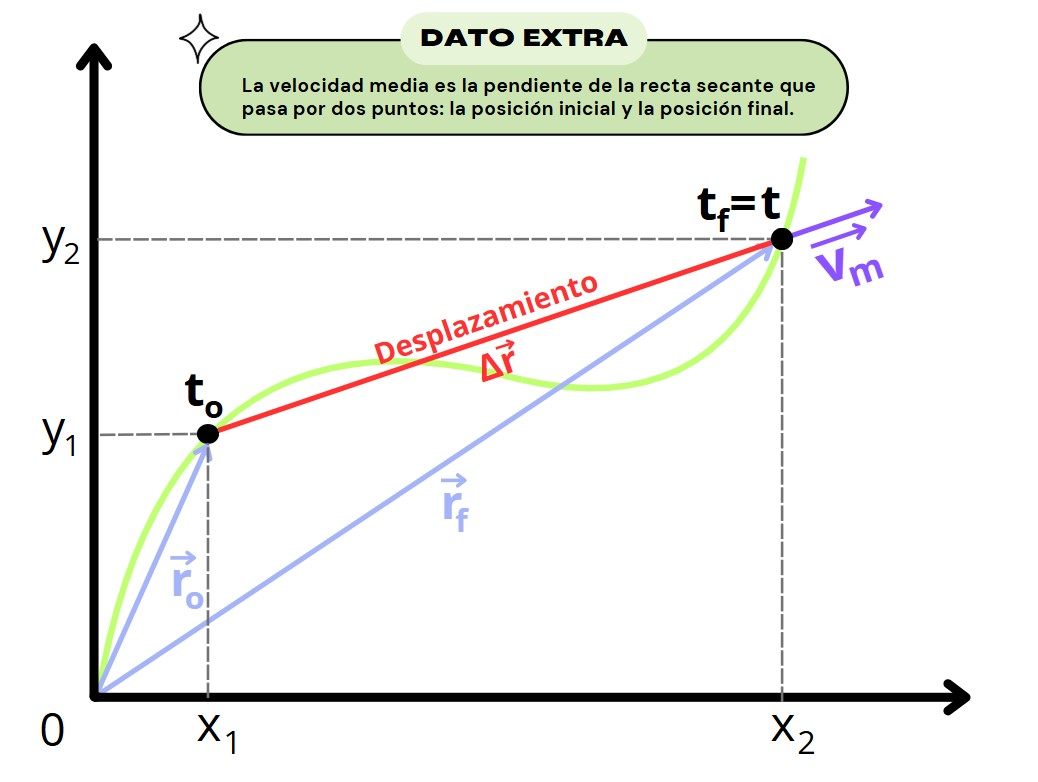
\includegraphics[width=0.6\textwidth]{images/cinematicGraphics/AverageSpeed.jpg}
    \caption{Representación gráfica de la velocidad media}
    \label{fig:velocidadMedia}
\end{figure}

\vspace{-40pt}

\[
\colorbox{blue!20}{$\displaystyle \vec{v}_m = \frac{\Delta \vec{r}}{\Delta t}$}
= \frac{\vec{r}_f - \vec{r}_o}{\vec{t}_f - \vec{t}_o}
\]

Su unidad en el Sistema Internacional es el metro por segundo (m/s).

\subsubsection{Velocidad instantánea}
La velocidad instantánea es la velocidad de un objeto en un instante preciso de tiempo. Se obtiene como el límite de la velocidad media cuando el intervalo de tiempo tiende a cero:

\begin{figure}[H]
    \centering
    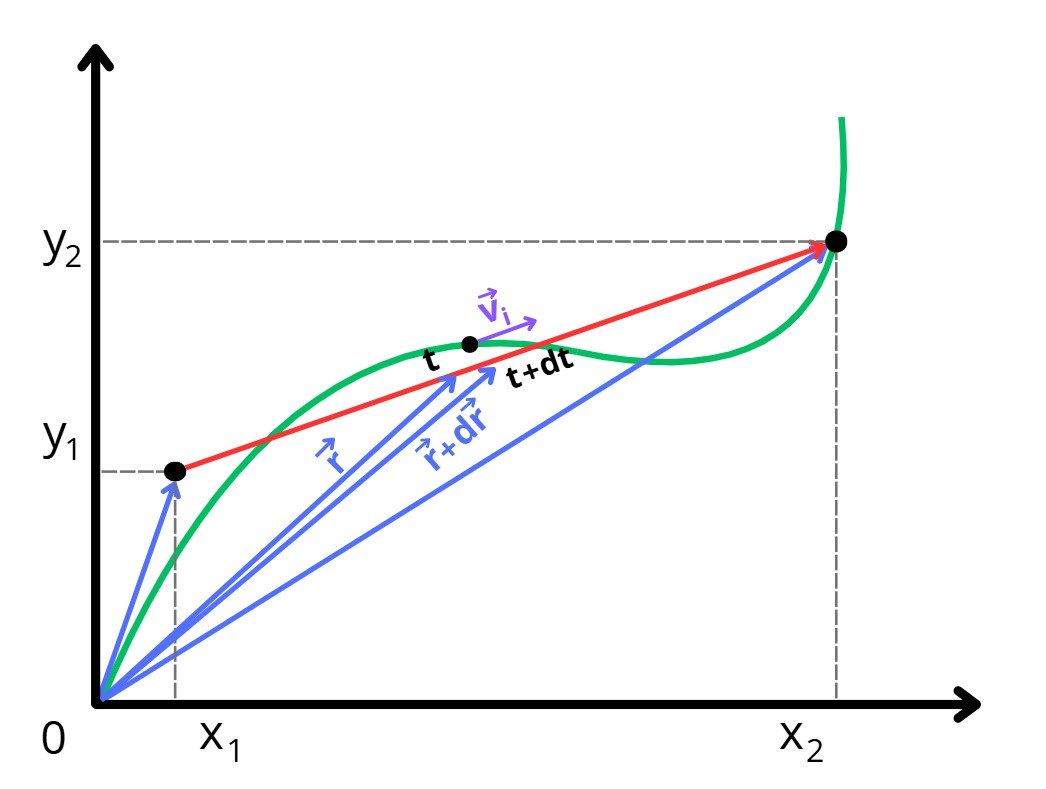
\includegraphics[width=0.6\textwidth]{images/cinematicGraphics/instantSpeed.jpg}
    \caption{Representación gráfica de la velocidad instantánea}
    \label{fig:velocidadInstantánea}
\end{figure}

\vspace{-40pt}

\[
\vec{v} = \lim_{\Delta t \to 0} \frac{\Delta \vec{r}}{\Delta t} = \frac{d\vec{r}}{dt}
\]

Geométricamente, corresponde a la pendiente de la recta tangente a la curva posición-tiempo en un punto dado.

\subsubsection{Ejemplo}

Encontrar a velocidad:

\begin{figure}[H]
    \centering
    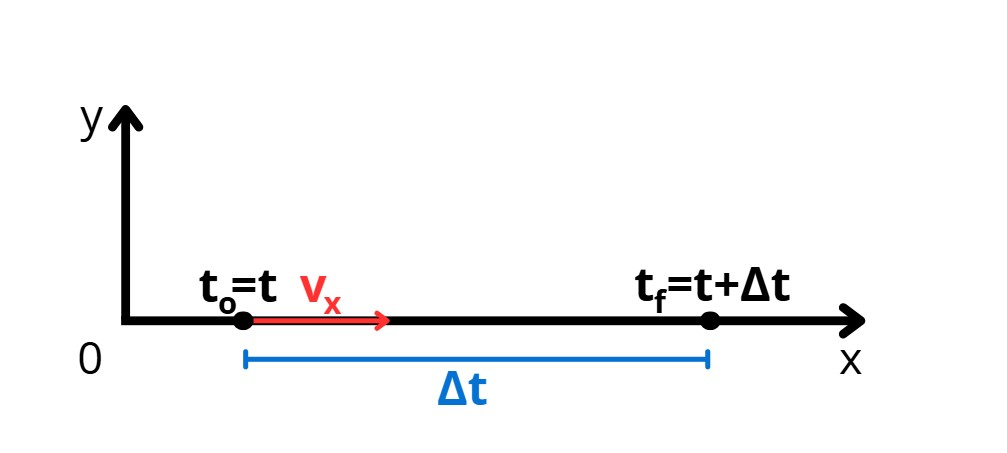
\includegraphics[width=0.6\textwidth]{images/demonstrations/example1.jpg}
    \caption{Representación gráfica del ejemplo 1}
    \label{fig:ejemplo1}
\end{figure}

\begin{align*}
&\textbf{Comprobación usando integrales:} \\
    \vec{v_x} &= \lim_{\Delta t \to 0} \frac{\Delta \vec{x}}{\Delta t} \\
    \vec{v_x} &= \lim_{\Delta t \to 0} \frac{x_f(t_f) - x_o(t_o)}{\Delta t} \\
&\text{Considerar } x(t) = t^2: \\    
    v_x &= \lim_{\Delta t \to 0} \frac{t_f^2 - t_o^2}{\Delta t} \\
    v_x &= \lim_{\Delta t \to 0} \frac{(t + \Delta t)^2 - t^2}{\Delta t} \\
    v_x &= \lim_{\Delta t \to 0} \frac{\cancel{t^2} + 2t\Delta t + (\Delta t)^2 - \cancel{t^2}}{\Delta t} \\
    v_x &= \lim_{\Delta t \to 0} \frac{\cancel{\Delta t}(2t + \Delta t)}{\cancel{\Delta t}} \\
    v_x &= \lim_{\Delta t \to 0} (2t + \cancel{\Delta t}) \\
    v_x &= 2t \\
&\textbf{Comprobación usando derivada:} \\
    v_x &= \frac{dx(t)}{dt} \\
    v_x &= \frac{d}{dt}(t^2) \\
    v_x &= 2t^{2-1} \\
    v_x &= 2t
\end{align*}

\[
\Rightarrow \quad \text{Ambos métodos coinciden.}
\]

\vspace{-20pt}

\subsection{Aceleración media e instantánea}

\begin{figure}[H]
    \centering
    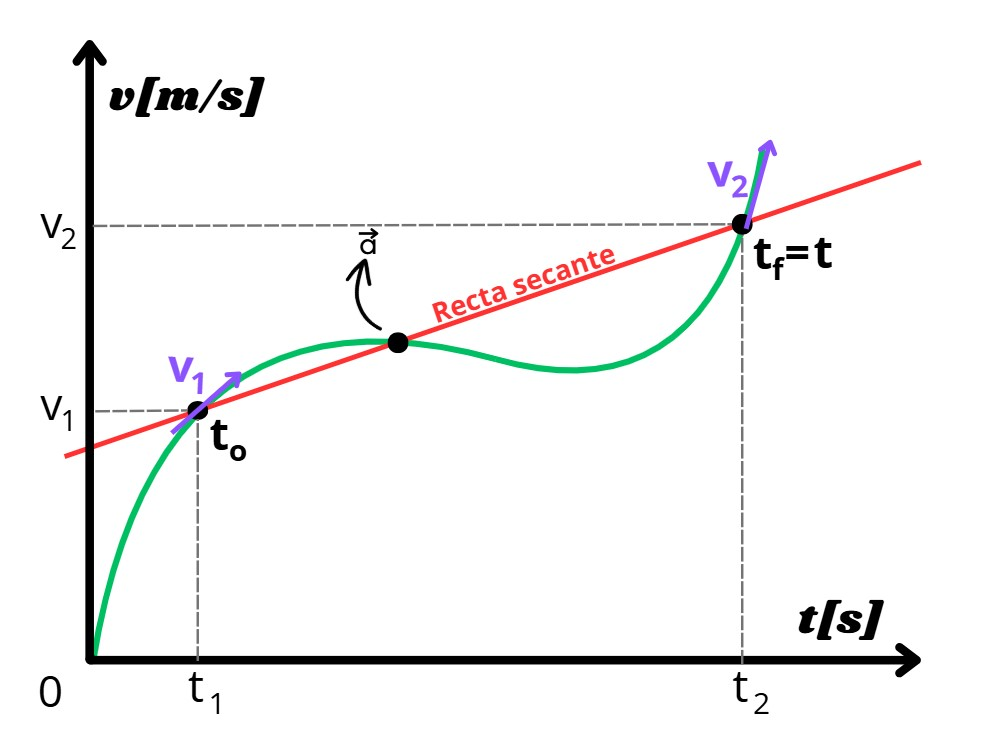
\includegraphics[width=0.6\textwidth]{images/cinematicGraphics/averageAcceleration.jpg}
    \caption{Representación gráfica de la Aceleración}
    \label{fig:Aceleración}
\end{figure}

\vspace{-20pt}

\[
[a] = [\frac{m/s}{s}] = [\frac{m}{s^2}]  \quad \text{S.I.} 
\]

\subsubsection{Aceleración media}
La aceleración media mide la variación de la velocidad en un intervalo de tiempo determinado:

\[
\vec{a}_m = \frac{\Delta \vec{v}}{\Delta t} = \frac{v_f - v_0}{t_f - t_0}
\]

\subsubsection{Aceleración instantánea}

La aceleración instantánea es la aceleración de un objeto en un instante preciso. Se define como el límite de la aceleración media cuando el intervalo de tiempo tiende a cero:

\begin{align*}
\vec{a} &= \lim_{\Delta t \to 0} (\frac{\Delta v}{\Delta t})\\
\vec{a} &= \frac{\Delta v}{\Delta t}(t) \\
\vec{a} &= \frac{d\vec{v}}{dt} \\
\vec{v} &= v_x \hat{\imath} + v_y \hat{\jmath} + v_z \hat{k} \\
\vec{a} &= \frac{d}{dt}(v_x \hat{\imath} + v_y \hat{\jmath} + v_z \hat{k}) \\
\vec{a} &= (\frac{dv_x}{dt})\hat{\imath} + (\frac{dv_y}{dt})\hat{\jmath} + (\frac{dv_z}{dt})\hat{k}
\end{align*}

\vspace{-10pt}

\begin{align*}
a_x &= \frac{dv_x}{dt}, \quad
a_y = \frac{dv_y}{dt}, \quad
a_z = \frac{dv_z}{dt}\\
\vec{a} &= a_x \hat{\imath} + a_y \hat{\jmath} + a_z \hat{k}\\
|\vec{a}| &= a = \sqrt{a_x^2 + a_y^2 + a_z^2}
\end{align*}

Geométricamente, corresponde a la pendiente de la recta tangente a la curva velocidad-tiempo en un punto dado.

\subsubsection{Ejemplo}

\begin{figure}[H]
    \centering
    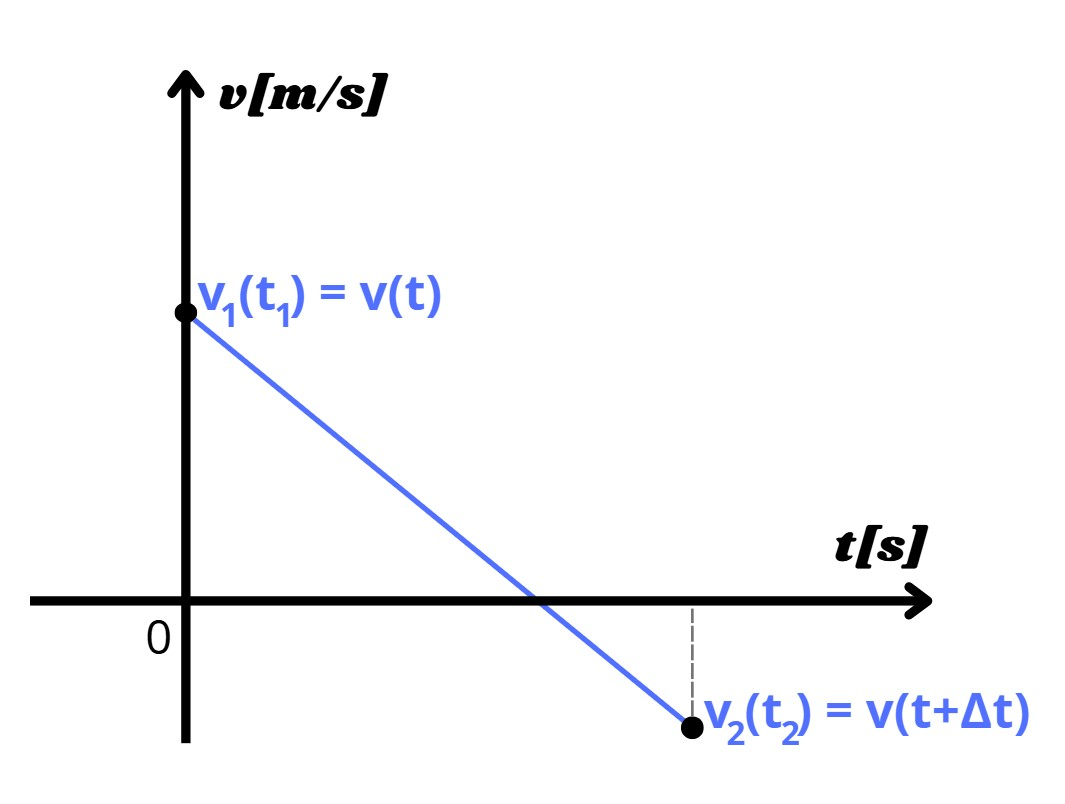
\includegraphics[width=0.6\textwidth]{images/demonstrations/example2.jpg}
    \caption{Representación gráfica del ejemplo 2}
    \label{fig:ejemplo 2}
\end{figure}

\begin{align*}
&\textbf{Comprobación usando integrales:} \\
    a_y &= \lim_{\Delta t \to 0} \frac{v_y(t+\Delta t) - v_y(t)}{\Delta t}
    \quad \text{con } v_{0y}=\text{ctte},\; g=9.8\,\text{m/s}^2 \\
    a_y &= \lim_{\Delta t \to 0} \left(\frac{\Delta v}{\Delta t}\right) \\
    a_y &= \lim_{\Delta t \to 0} \left(\frac{v(t_2) - v(t_1)}{\Delta t}\right) \\
    a_y &= \lim_{\Delta t \to 0} \left(\frac{(v_{0y} - gt_2)-(v_{0y} - gt_1)}{\Delta t}\right) \\
    a_y &= \lim_{\Delta t \to 0} \frac{[v_{0y} - g(t+\Delta t)] - [v_{0y} - gt]}{\Delta t} \\
    a_y &= \lim_{\Delta t \to 0} \frac{\cancel{v_{0y}} - \cancel{gt} - g\Delta t - \cancel{v_{0y}} + \cancel{gt}}{\Delta t} \\
    a_y &= \lim_{\Delta t \to 0} \frac{-g\cancel{\Delta t}}{\cancel{\Delta t}} \\
    a_y &= \lim_{\Delta t \to 0} (-g) \\
    a_y &= -g \\
&\textbf{Comprobación usando derivada:} \\
    \vec{a} &= \frac{dv(t)}{dt} \\
    \vec{a} &= \frac{d}{dt}(v_{0y}-gt) \\
    \vec{a} &= \frac{d}{dt}(\cancel{v_{0y}}) - \frac{d}{dt}(gt)\\
    \vec{a} &= -g \cancel{\frac{dt}{dt}}\\
    a &= -g
\end{align*}

%%%%%%%%%%%%%%%%%%%%%

%%%%%%%%%%%%%%%%%%%%%
\section{Movimiento uniforme}

\subsection{Definición}
El movimiento uniforme es aquel en el cual la velocidad es constante en el tiempo.

\vspace{-20pt}

\begin{align*}
\vec{v}_x = \text{cte} \quad \Rightarrow \quad \vec{a} = 0
\end{align*}

\vspace{-20pt}

\subsection{Velocidad}
\begin{align*}
\vec{v}_x &= \frac{\Delta \vec{x}}{\Delta t} \\
\Delta \vec{x} &= \vec{v}\,\Delta t
\end{align*}

Si $\Delta t$ es constante, entonces también $\Delta x$ es constante.

\vspace{-10pt}

\subsection{Ecuación de movimiento}

\vspace{-30pt}

\begin{align*}
\vec{x}_f - \vec{x}_0 &= \vec{v}_x (t_f - \cancel{t_0}) \\
\text{Tomando } t_f = t: \\
\vec{x}_f &= \vec{x}_0 + \vec{v}_x t \quad \text{(ecuación vectorial)} \\
x &= x_0 + v_x t \quad \text{(ecuación escalar)}
\end{align*}

\subsection{Interpretación gráfica}

\begin{figure}[H]
    \centering
    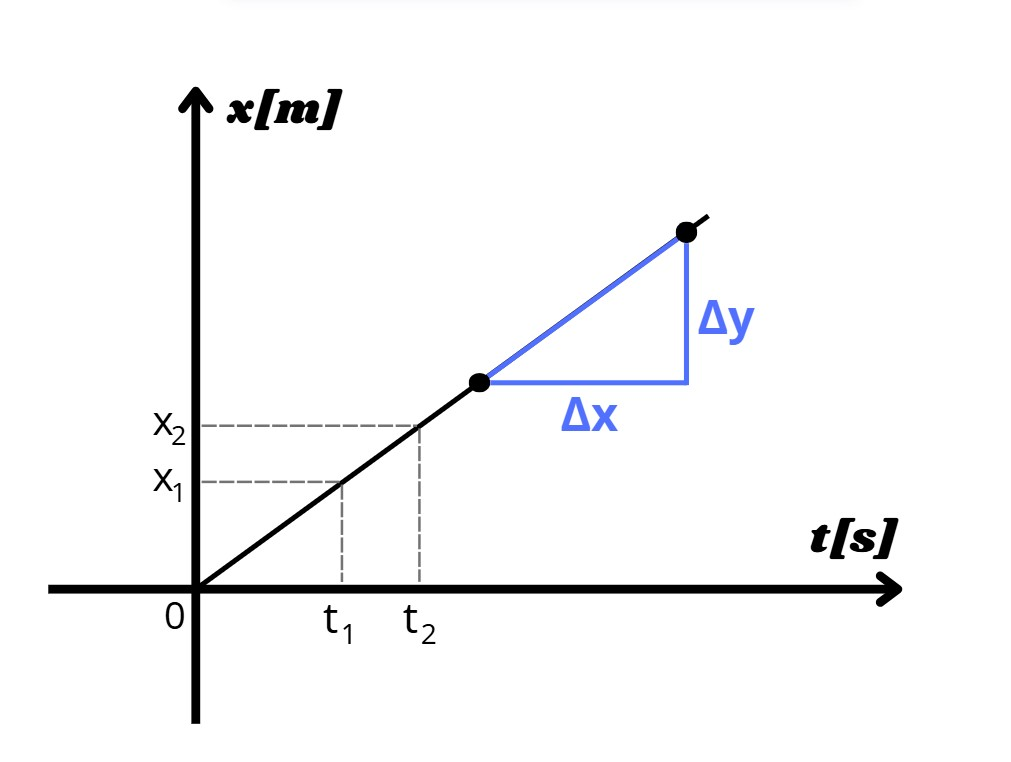
\includegraphics[width=0.6\textwidth]{images/demonstrations/uniformMovement.jpg}
    \caption{Representación gráfica del movimiento uniforme}
    \label{fig:movimiento uniforme}
\end{figure}

La ecuación es de la forma:
\vspace{-20pt}

\begin{align*}
\vec{r} &= \vec{r_0} + \vec{v}t\\
y &= A + Bx
\end{align*}

Donde:
\begin{itemize}
\item $A$ es la ordenada en el origen ($x_0$)
\item $B$ es la pendiente ($v = \frac{\Delta x}{\Delta t}$)
\end{itemize}

%%%%%%%%%%%%%%%%%%%%%

%%%%%%%%%%%%%%%%%%%%%
\section{Cinematica de la particula}
\vspace{-20pt}
\begin{align*}
\vec{v_m} &= \lim_{\Delta t \to 0} \left(\frac{\Delta \vec{r}}{\Delta t}\right)\\
          &\colorbox{blue!20}{$\vec{v_m} = \frac{d\vec{r}}{dt}(t)$} \\
\vec{a_m} &= \lim_{\Delta t \to 0} \left(\frac{\Delta \vec{v}}{\Delta t}\right)\\
          &\colorbox{blue!20}{$\vec{a} = \frac{d\vec{v}}{dt}(t)$}
\end{align*}

\text{Ecuaciones en forma integral}
\vspace{-20pt}

\begin{align*}
v &= \frac{dr}{dt}(t) \\
\int dr &= \int v(t)\, dt \\
a &= \frac{dv}{dt}(t) \\
\int dv &= \int a(t)\, dt
\end{align*}

%%%%%%%%%%%%%%%%%%%%%

%%%%%%%%%%%%%%%%%%%%%
\section{Cálculo diferencial}

El cálculo diferencial estudia cómo cambian las funciones. Sus herramientas principales son las derivadas, que permiten analizar la variación instantánea de una magnitud.

\subsection{Derivadas}

La derivada de una función mide la tasa de cambio instantánea. Se define como:

\begin{figure}[H]
    \centering
    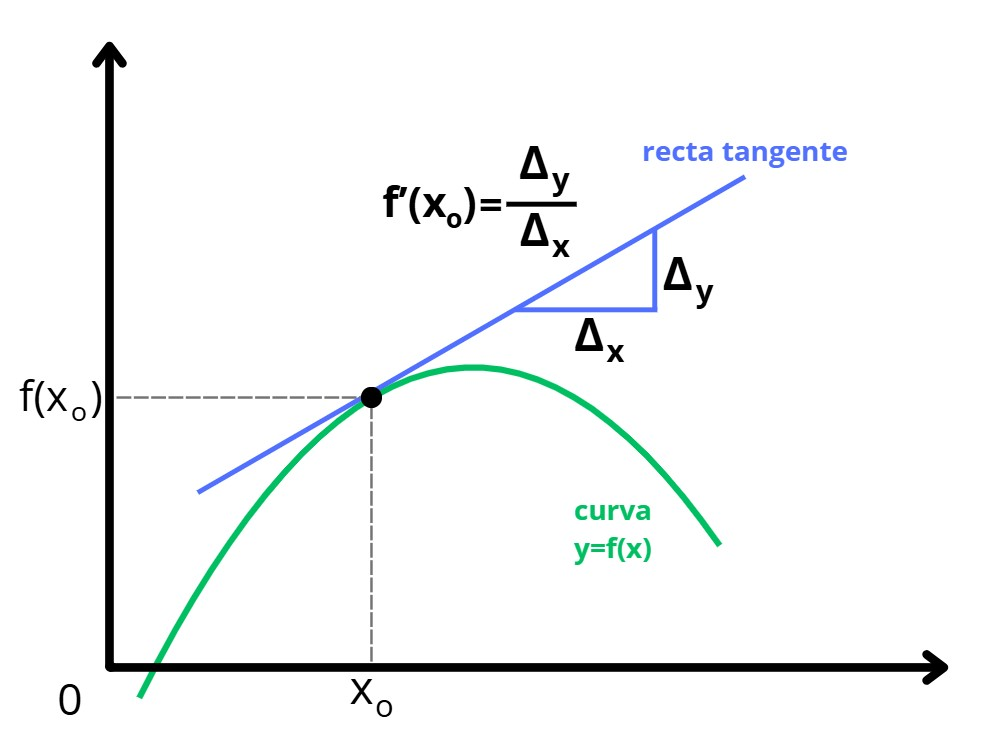
\includegraphics[width=0.6\textwidth]{images/cinematicGraphics/derivative.jpg}
    \caption{Representación gráfica de la derivada}
    \label{fig:derivada}
\end{figure}

\vspace{-40pt}

\[
f'(x) = \lim_{\Delta x \to 0} \frac{f(x+\Delta x) - f(x)}{\Delta x}
\]

\subsubsection{Interpretación}

Geométricamente, la derivada representa la pendiente de la recta tangente a la curva en un punto.

Físicamente, por ejemplo:
\[
v = \frac{dx}{dt}
\]
representa la velocidad como cambio de posición respecto al tiempo.

\subsubsection{Reglas de derivación}

Las reglas de derivación permiten calcular derivadas de manera rápida sin usar directamente la definición.

\begin{itemize}

\item \textbf{Regla de la suma:}

\[
\frac{d}{dx}[f(x) + g(x)] = \frac{df}{dx} + \frac{dg}{dx}
\]

\textbf{Ejemplo:}
\[
\frac{d}{dx}(x^2 + x) = \frac{d}{dx}(x^2) + \frac{d}{dx}(x) = 2x + 1
\]

\item \textbf{Regla del producto:}

\[
\frac{d}{dx}[f(x)g(x)] = f'(x)g(x) + f(x)g'(x)
\]

\textbf{Ejemplo:}
\[
\frac{d}{dx}(x^2 \cdot x) = \frac{d}{dx}(x^2)\cdot x + x^2 \cdot \frac{d}{dx}(x)
\]
\[
= 2x \cdot x + x^2 \cdot 1 = 2x^2 + x^2 = 3x^2
\]

\item \textbf{Regla del cociente:}

\[
\frac{d}{dx}\left[\frac{f(x)}{g(x)}\right] = \frac{f'(x)g(x) - f(x)g'(x)}{g(x)^2}
\]

\textbf{Ejemplo:}
\[
\frac{d}{dx}\left(\frac{x^2}{x}\right)
= \frac{\frac{d}{dx}(x^2)\cdot x - x^2 \cdot \frac{d}{dx}(x)}{x^2}
\]
\[
= \frac{2x \cdot x - x^2 \cdot 1}{x^2}
= \frac{2x^2 - x^2}{x^2} = 1
\]

\item \textbf{Regla de la cadena:}

\[
\frac{d}{dx}f(g(x)) = f'(g(x)) \cdot g'(x)
\]

\textbf{Ejemplo:}
\[
\frac{d}{dx}(x^2 + 1)^2 = \frac{d}{dx}\left[(x^2 + 1)^2\right]
\]
\[
= 2(x^2 + 1)\cdot \frac{d}{dx}(x^2 + 1)
\]
\[
= 2(x^2 + 1)\cdot (2x) = 4x(x^2 + 1)
\]

\end{itemize}

\subsubsection{Derivadas básicas}

\begin{itemize}

\item Potencia:
\[
\frac{d}{dx}(x^n) = nx^{n-1}
\]

\textbf{Ejemplo:}
\[
\frac{d}{dx}(x^3) = 3x^2
\]

\item Seno:
\[
\frac{d}{dx}(\sin x) = \cos x
\]

\item Coseno:
\[
\frac{d}{dx}(\cos x) = -\sin x
\]

\item Exponencial:
\[
\frac{d}{dx}(e^x) = e^x
\]

\end{itemize}

\subsection{Integrales}

La integral es la operación inversa de la derivada y permite calcular áreas bajo la curva.

\subsubsection{Integral indefinida}

\begin{figure}[H]
    \centering
    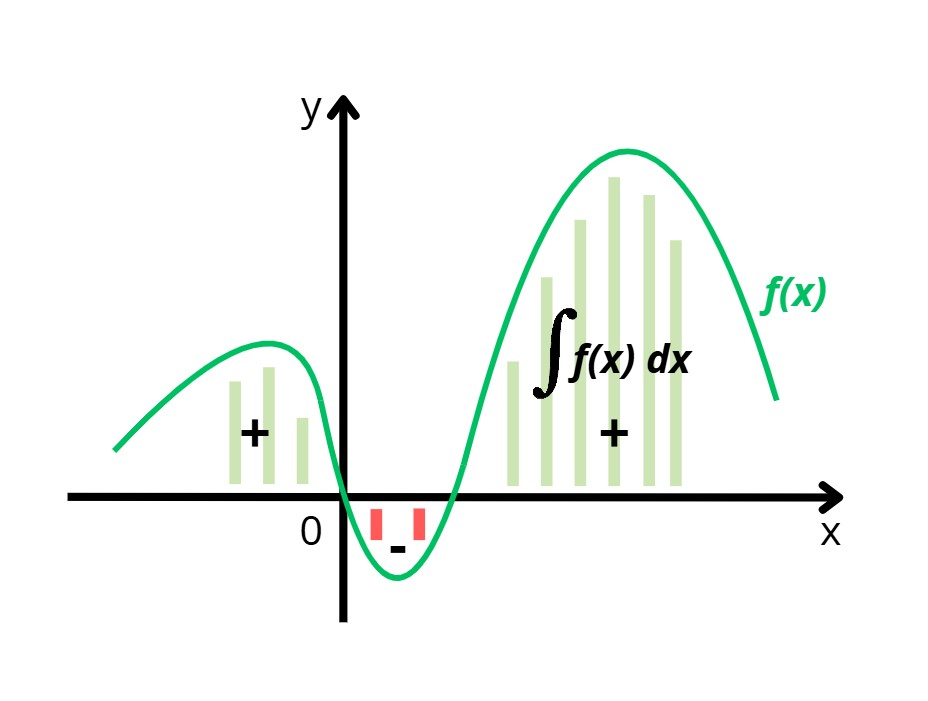
\includegraphics[width=0.6\textwidth]{images/cinematicGraphics/indefiniteIntegral.jpg}
    \caption{Representación gráfica de la integral indefinida}
    \label{fig:intregral indefinida}
\end{figure}

\vspace{-40pt}

\[
\int f(x)\,dx = F(x) + C
\]

donde $F'(x) = f(x)$, es decir, $F(x)$ es una función cuya derivada es $f(x)$.

\textbf{Ejemplo:}
\[
\int 2x \, dx = x^2 + C
\]

porque:
\[
\frac{d}{dx}(x^2) = 2x
\]


\subsubsection{Integral definida}

\begin{figure}[H]
    \centering
    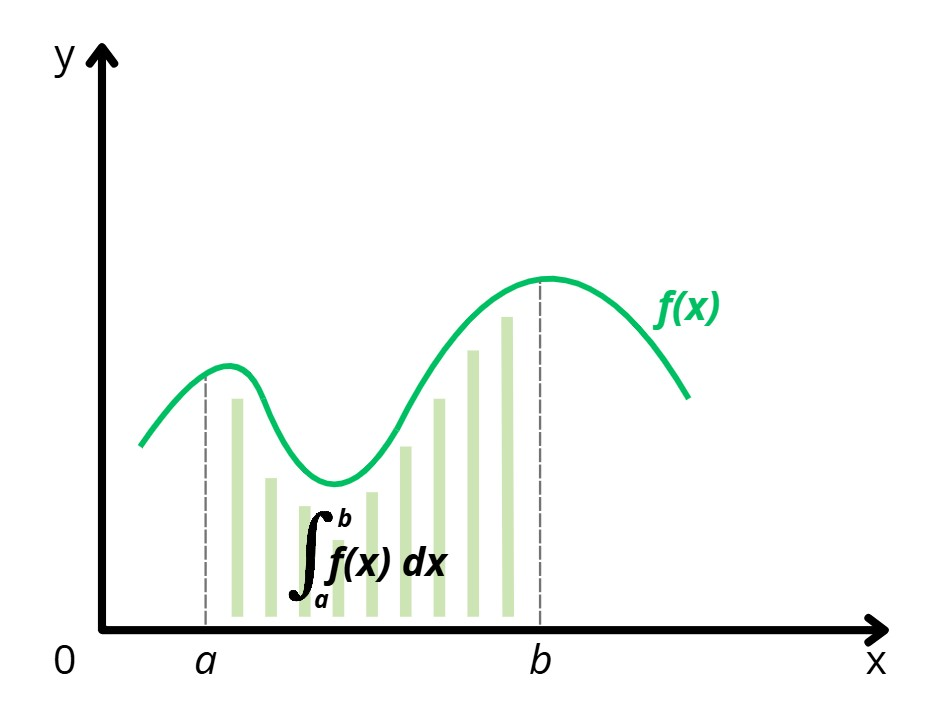
\includegraphics[width=0.6\textwidth]{images/cinematicGraphics/definiteIntegral.jpg}
    \caption{Representación gráfica de la integral definida}
    \label{fig:intregral definida}
\end{figure}

\vspace{-40pt}

\[
\int_a^b f(x)\,dx
\]

representa el área bajo la curva entre $a$ y $b$.

\textbf{Ejemplo:}
\[
\int_0^2 x \, dx
\]

Primero encontramos una primitiva:
\[
\int x \, dx = \frac{x^2}{2}
\]

Luego evaluamos en los límites:
\[
\left[\frac{x^2}{2}\right]_0^2 = \frac{2^2}{2} - \frac{0^2}{2}
\]
\[
= \frac{4}{2} - 0 = 2
\]

\subsubsection{Reglas de integración}

\begin{itemize}

\item \textbf{Regla de la potencia:}
\[
\int x^n dx = \frac{x^{n+1}}{n+1} + C
\]

\[
\int x^2 dx = \frac{x^3}{3} + C
\]

\item \textbf{Integral del coseno:}
\[
\int \cos x \, dx = \sin x + C
\]

\item \textbf{Integral del seno:}
\[
\int \sin x \, dx = -\cos x + C
\]

\end{itemize}

%%%%%%%%%%%%%%%%%%%%%

%%%%%%%%%%%%%%%%%%%%%
\section{Movimiento Rectilíneo Uniforme (MRU)}



El Movimiento Rectilíneo Uniforme (MRU) es aquel en el que un objeto se desplaza en línea recta con velocidad constante, es decir, con aceleración igual a cero.

\[
a = 0 \qquad v = \text{constante}
\]

\subsection{Ecuación de posición}

{v} = \text{ctte} \quad \text{la velocidad no es función del tiempo}
\begin{align*}
\text{* la ecuación integral}\\
\int_{x_0}^{x} dx &= \int_{t_0}^{t} v(t)\, dt\\
\text{* si } v(t)=\text{ctte}=v\\
\int_{x_0}^{{x^0}} {x^0} dx &= v \int_{t_0}^{t} {t^0} dt\\
\left[\frac{1}{0+1}x^{0+1} \right]_{x_0}^{x} &= v\left[\frac{1}{0+1}t^{0+1}\right]_{t_0}^{t}\\
[x]_{x_0}^{x} &= v[t]_{t_0}^{t}\\
x - x_0 &= v(t - \cancel{t_0})\\
\end{align*}

\vspace{-60pt}

\[
\hspace{1,8cm}\colorbox{blue!20}{$\vec{x}(t) = \vec{x}_0 + \vec{v}t$}
\]
Donde $x_0$ es la posición inicial, $v$ es la velocidad constante y $t$ es el tiempo transcurrido.

\subsection{Características del MRU}

\begin{itemize}
    \item La trayectoria es una línea recta.
    \item La velocidad se mantiene constante en módulo, dirección y sentido.
    \item La aceleración es cero.
    \item El desplazamiento es proporcional al tiempo.
\end{itemize}


%%%%%%%%%%%%%%%%%%%%%

%%%%%%%%%%%%%%%%%%%%%
\section{Movimiento Rectilíneo Uniformemente Variado (MRUV)}

El Movimiento Rectilíneo Uniformemente Variado (MRUV) se caracteriza por presentar una aceleración constante distinta de cero. En este tipo de movimiento, la velocidad cambia de manera uniforme con respecto al tiempo.

\subsection{Ecuaciones}

\[
a=\text{cte} \;\Rightarrow\; v \neq \text{cte}
\]

\vspace{-20pt}

Primera ecuacion:
\begin{align*}
a &= \frac{dv}{dt}\\
dv &= a\,dt\\
\int_{v_0}^{v} dv &= \int_{0}^{t} a\,dt\\
\left[v\right]_{v_0}^{v} &= a\left[t\right]_{0}^{t}\\
v - v_0 &= a(t-0)
\end{align*}

\vspace{-20pt}

\[
\colorbox{blue!20}{$v = v_0 + at$}
\]

Segunda ecuacion:

\begin{align*}
v &= \frac{dx}{dt}\\
dx &= v(t)\,dt\\
\int_{x_0}^{x} dx &= \int_{0}^{t} (v_0 + at)\,dt\\
\int_{x_0}^{x} dx &= \int_{0}^{t} v_0\,dt + \int_{0}^{t} at\,dt\\
\left[x\right]_{x_0}^{x} &= v_0\left[t\right]_{0}^{t} + a\left[\frac{t^2}{2}\right]_{0}^{t}\\
x - x_0 &= v_0(t-0) + \frac{1}{2}a(t^2-0)
\end{align*}

\vspace{-20pt}

\[
\colorbox{blue!20}{$x = x_0 + v_0 t + \frac{1}{2}at^2$}
\]

Tercera ecuacion:

\begin{align*}
a &= \frac{dv}{dt}\\
dv &= a dt\\
dv &= a dt(\frac{dx}{dx})\\
dv &= \frac{a dx}{(\frac{dx}{dt})}\\
dv &= a\frac{dx}{v}\\
v\,dv &= a\,dx\\
\int_{v_0}^{v} v\,dv &= \int_{x_0}^{x} a\,dx\\
\left[\frac{v^2}{2}\right]_{v_0}^{v} &= a\left[x\right]_{x_0}^{x}\\
\frac{1}{2}(v^2 - v_0^2) &= a(x - x_0)
\end{align*}

\vspace{-20pt}

\[
\colorbox{blue!20}{$v^2 = v_0^2 + 2a(x - x_0)$}
\]


Las ecuaciones fundamentales del MRUV son:

\begin{itemize}
    \item Ecuación de posición:
    \[
    x = x_0 + v_0 t + \frac{1}{2}at^2
    \]

    \item Ecuación de velocidad:
    \[
    v = v_0 + at
    \]

    \item Ecuación independiente del tiempo:
    \[
    v^2 = v_0^2 + 2a(x - x_0)
    \]
\end{itemize}

Donde:
\begin{itemize}
    \item $x$: posición final
    \item $x_0$: posición inicial
    \item $v$: velocidad final
    \item $v_0$: velocidad inicial
    \item $a$: aceleración
    \item $t$: tiempo
\end{itemize}

\subsection{Características del MRUV}

\begin{itemize}
    \item La trayectoria es una línea recta.
    \item La aceleración es constante y distinta de cero.
    \item La velocidad cambia de manera uniforme con el tiempo.
    \item La gráfica posición-tiempo es una parábola.
    \item La gráfica velocidad-tiempo es una línea recta con pendiente igual a la aceleración.
    \item Si la aceleración es positiva, el objeto acelera; si es negativa, desacelera.
\end{itemize}



%%%%%%%%%%%%%%%%%%%%%

%%%%%%%%%%%%%%%%%%%%%
\section{Simulación}

\subsection{Materiales}

\begin{itemize}
    \item Computadora o laptop
    \item Software GeoGebra
    \item Cuaderno de apuntes
\end{itemize}

\subsection{Procedimiento}

\begin{enumerate}
    \item Abrir el software GeoGebra.
    \item Definir la función de posición:
    \[
    x(t) = x_0 + v_0 t + \frac{1}{2}at^2
    \]
\end{enumerate}

\subsection{Resultados}

A partir de la simulación realizada en GeoGebra se obtuvieron los siguientes resultados:

\begin{itemize}
    \item La gráfica obtenida muestra\ldots
\end{itemize}

\begin{table}[H]
\centering
\begin{tabular}{c|c|c}
Tiempo (s) & Posición (m) & Velocidad (m/s) \\\hline
0 & 0 & 2 \\
1 & 2.5 & 3 \\
\end{tabular}
\caption{Datos obtenidos en la simulación}
\end{table}

\subsection{Análisis}

Los resultados obtenidos permiten observar que\ldots

\subsection{Conclusiones}

\begin{itemize}
    \item 
\end{itemize}

\subsection{Recomendaciones}

\begin{itemize}
    \item 
\end{itemize}